\subsection{Estructura del paradigma}

La programación dinámica es famosa por su ubicuidad e infame por su dificultad. Su dificultad radica en que requiere modelar el problema de una forma muy particular. Esta sección intenta desglosar la estructura del paradigma para dar sentido a esa forma de modelar.

\subsubsection{Propiedades del problema}

Para poder aplicar el paradigma, el problema debe tener dos propiedades:
\begin{enumerate}
    \item Es posible dividirlo en subproblemas cuyas soluciones permiten construir una solución al problema original.
    \begin{itemize}
        \item Tradicionalmente, esa propiedad se redacta orientada a problemas de optimización y se denomina \concept{subestructura óptima}: la solución óptima del problema original se puede construir a partir de soluciones óptimas a sus subproblemas.
    \end{itemize} 
    \item \concept{Subproblemas superpuestos}: Varios subproblemas tienen subsubproblemas repetidos, de forma que un algoritmo recursivo acabaría resolviendo los mismos subsubproblemas varias veces.
    % Esto de abajo es verdad, pero, para qué lo estoy diciendo?
    % \begin{itemize}
    %     \item Para que eso ocurra, el espacio de posibles subproblemas debe ser pequeño, usualmente polinomial en el tamaño de la entrada. De lo contrario, es posible que no hayan subproblemas repetidos.
    % \end{itemize}
\end{enumerate}

Si el problema no tiene esas propiedades, no tiene sentido intentar resolverlo con un algoritmo de programación dinámica: si no es posible construir la solución a partir de la de sus subproblemas, no sirve de nada resolverlos, no aplica el paradigma; y sin subproblemas superpuestos, almacenar los subproblemas no trae ningún beneficio, pues no se reutilizan las soluciones.

\subsubsection{Tipos de programación dinámica}

Hay en esencia dos formas de diseñar algoritmos de programación dinámica: 
\begin{itemize}
    \item \concept{\textit{Top-down}} (del problema más general a los más pequeños): Se resuelve el problema original de forma recursiva, pero cada vez que se resuelve un subproblema, se \concept{memoiza}%
    %
    \footnote{El término \say{memoización} (no \say{memorización}) proviene del artículo de \textcite{michie_memo} en el que se explica cómo convertir funciones recursivas a \say{funciones memo}, que reutilizan resultados ya computados en lugar de hacer llamados recursivos.}%
    %
    : se almacena el resultado de cada llamado recursivo en una estructura de datos externa a la función recursiva para evitar tener que recomputarlo.
    \item \concept{\textit{Bottom-up}} (de los problemas pequeños al general): Se resuelven primero los subproblemas más pequeños y se almacenan sus resultados en una tabla. Esas soluciones se usan para ir completando la tabla iterativamente con las soluciones a subproblemas más grandes, hasta la solución del problema original. A eso se le denomina \concept{tabulación}.
\end{itemize}

Como ambos métodos aprovechan la propiedad de subproblemas superpuestos, sus complejidades asintóticas suelen ser iguales. Sin embargo, cuando \textit{todos} los subproblemas posibles se tienen que resolver al menos una vez, el algoritmo bottom-up suele ser más eficiente que el top-down por un factor constante, porque el algoritmo top-down tiene el \hyperref[sec:sobrecosto_recursion]{sobrecosto de la recursión}.

Ocasionalmente, solo es necesario resolver algunos de los posibles subproblemas; en ese caso, la solución top-down es mejor porque solo resuelve y memoiza los subproblemas que sí se tienen que resolver, mientras que la bottom-up requiere resolver los subproblemas pequeños primero para completar la tabulación.

\subsubsection{Modelos del problema}

Para resolver un problema mediante programación dinámica, se debe modelar de forma que sea compatible con el paradigma. En particular, se acostumbra definir:
\begin{enumerate}
    \item \concept{Estados}: Se identifican las variables del problema que satisfacen que si alguna cambia, se tiene un subproblema distinto. Cada combinación de valores de esas variables define un \concept{estado} del problema.
    \item \concept{Relación de recurrencia}: Una ecuación que expresa la solución asociada a un estado (a un subproblema) en términos de las soluciones asociadas a otros estados (a otros subproblemas).
\end{enumerate}

A partir de esas dos cosas, la implementación top-down es mecánica: se utiliza la relación de recurrencia para hacer una implementación recursiva y se le añade memoización (lo cual es simple: crear la estructura externa y almacenar en ella el resultado de cada llamado recursivo).

La implementación bottom-up no sigue el orden de la relación de recurrencia, sino un orden inverso. Por ende, para implementarla, hace falta saber en qué orden realizar la tabulación tal que al intentar resolver un subproblema, los subsubproblemas de los que depende ya estén resueltos. Eso se visualiza mediante un grafo de dependencias:
\begin{enumerate}
    \setcounter{enumi}{2}
    \item \concept{Grafo de dependencias} (\textit{Dependency DAG}): Un grafo acíclico dirigido donde cada vértice representa un estado y cada arco \(u \longrightarrow v\) representa que la solución a \(u\) es necesaria para computar la de \(v\).

    Con eso, se puede seguir cualquier orden topológico del grafo (cualquiera en el que todo vértice aparece después de sus predecesores) para tabular.
\end{enumerate}

Más aún, el grafo de dependencias muestra que muchas veces no se necesitan las soluciones a todos los subproblemas anteriores para calcular el siguiente, sino solo las de algunos, lo que permite olvidar algunas soluciones en cierto punto y mejorar la complejidad espacial del algoritmo.

\subsubsection{Estructura del paradigma}

El grafo dirigido de la figura \ref{fig:programacion_dinamica} muestra la relación entre los modelos que se realizan para el problema y los algoritmos que habilitan, donde los arcos denotan dependencia.

\usetikzlibrary{arrows.meta}
\begin{figure}[htb]
\centering
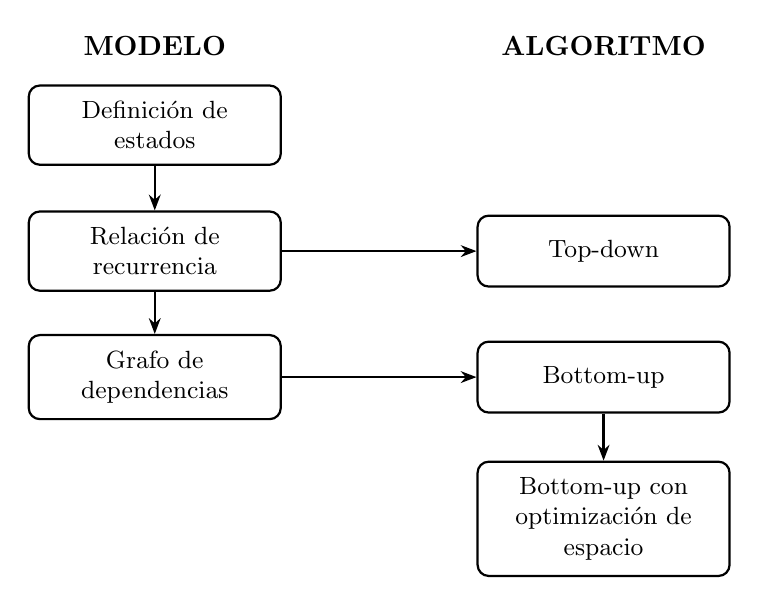
\begin{tikzpicture}[
    font=\small,
    x=1mm, y=1mm,
    box/.style={
        rectangle, draw, thick, rounded corners,
        align=center, minimum width=32mm, minimum height=9mm,
        inner sep=2mm
    },
    header/.style={font=\bfseries},
    conn/.style={-{Stealth[length=2mm]}, thick},
]

    % Column x-coordinates: a wide gap separates MODELO from ALGORITMO.
    \def\xModelo{0}
    \def\xEstrategia{57}

    % Row y-coordinates.
    \def\yUno{0}
    \def\yDos{-16}
    \def\yTres{-32}
    \def\yCuatro{-50}

    % ---------- MODELO (left column) ----------
    \node[box] (estados) at (\xModelo, \yUno) {Definición de\\estados};
    \node[box] (recurrencia) at (\xModelo, \yDos) {Relación de\\recurrencia};
    \node[box] (grafo) at (\xModelo, \yTres) {Grafo de\\dependencias};

    \draw[conn] (estados) -- (recurrencia);
    \draw[conn] (recurrencia) -- (grafo);

    % ---------- ALGORITMO: estrategia de evaluación ----------
    \node[box] (topdown) at (\xEstrategia, \yDos) {Top-down};
    \node[box] (bottomup) at (\xEstrategia, \yTres) {Bottom-up};
    \node[box] (bottomup-opt) at (\xEstrategia, \yCuatro) {Bottom-up con\\optimización de\\espacio};

    \draw[conn] (recurrencia) -- (topdown);
    \draw[conn] (grafo) -- (bottomup);
    \draw[conn] (bottomup) -- (bottomup-opt);

    % ---------- Headers ----------
    \node[header] (modelo-header) at (\xModelo, 10) {MODELO};
    \node[header] (algoritmo-header) at (\xEstrategia, 10) {ALGORITMO};

\end{tikzpicture}
\caption{Elementos del modelo de un problema de programación dinámica y del algoritmo que lo resuelve.}
\label{fig:programacion_dinamica}
\end{figure}


una vez se tienen esos modelos matemáticos, la implementación de los algoritmos de programación dinámica es netamente procedimental: ya no hace falta pensar más sobre el problema, solo plasmar los modelos en el código.

Se presentan varios ejemplos para concretar estas ideas: tanto para ilustrar cómo se modela el problema como para demostrar que, dados los modelos, escribir los algoritmos es automático.
